\documentclass[10pt, a4paper]{article}
\usepackage[utf8]{inputenc}
\usepackage{multirow}
\usepackage{graphicx}
\usepackage[backend=biber, style=numeric, sorting=ynt]{biblatex}

\addbibresource{ref.bib}

\title{Information Processing and the Brain CW 2}
\author{Kheeran Naidu}
\date{December 2019}

\begin{document}
\maketitle

\section*{Introduction}
For CW2, I have decided to implement and explore the behaviour of the classical \textit{Reinforcement Learning} algorithm using \textit{Temporal Difference Learning}. Reinforcement learning (RL) was developed from an area of psychology of animal lerning under the name trial-and-error learning \cite{woodworth1937experimental} and the area of the optimal control problem - using value functions and dynamic programming - in the form of Markov Decision Processes \cite{bellman1957markov}\cite{bellman1957dynamic}. Temporal-difference (TD) methods for RL were proposed as a model of classical (or Pavlovian) conditioning in 1987 \cite{sutton1987temporal}, and refined to the TD learning rule in 1990 \cite{sutton1990time}. Put simply, RL is the computational method for goal-oriented learning and the TD learning rule is one which is based on the difference in the current state value and next state value.

\section*{Question 1}
The RL algorithm is based on the formal framework of Markov decision processes. A Markov decision process is a 4-tuple $(S,A,P_a, R_a)$ that models an environment where $S =$ the set of states, $A =$ the set of actions, $P_a(s,s')$ the transition probability of the action $a$ taking state $s$ to $s'$ and $R_a(s,s')$ the reward function of the action $a$ which takes state $s$ to $s'$. We often include a discount factor $\gamma \in [0,1]$ to discount future rewards. In the algorithm, we will exlpoit the Markovian property that the probability of being in a state $s_{t+1}$ with reward $R_a(s_t, s_{t+1})$ at time $t+1$ is completely described by the state $s_t$ and action $a_t$ at time $t$, independent of states and actions before time $t$.

In this CW2 the environment is represented by the $6 \times 8$ grid world with walls as obstacles and a single terminal state with reward of 1. In this finite world, the goal is for the agent to obtain the highest reward by following an optimal policy (the actions to take at a particular state) of moving through the environment, which turns out to be the shortest path to the terminal state. Figure \ref{} represents the grid world where each non-walled tile of the grid is a state and the set of actions are $\{up, down, left, right\}$ which move to the respective adjacent non-walled tiles.


\section*{Question 2}
The RL algorithm is highly relatable to areas of the brain such as the dopaminergic systems \cite{roelfsema2018control} which code for unexpected reward. Recent views discuss the significant role of the neurotransmitter dopamine in  goal-directed behavior, cognition, attention, and reward \cite{schultz2002getting}.

\section*{Question 3}


\section*{Question 4}
It has been shown that novel sensory stimuli induce similar activity of dopamine cells on unpredicted rewards \cite{kakade2002dopamine}. The difference being that as the stimuli becomes familiar, the activity diminishes. This has been reasoned by the fact that novelty itself has rewarding characteristics \cite{reed1996intrinsic} and is intrinsically motivated \cite{dayan2002reward}. The algorithm we have used is a solely extrinsically motivated method of RL, it doesn't cater for the intrinsically motivated rewards that biologcally occurs in animals. Biologically, this intrinsic motivation encourages exploration of an environment which in our algorithm is modelled by the epsilon-greedy mechanism of taking a random action with probability $\epsilon$. However, this approach isn't motivated by the novelty of a stimuli (or state in our case). 

Sutton and Barto identify this shortcomming of RL and note that an animal's reward signals are determined by processes within its brain that monitor both the external state and animal's internal state \cite{sutton1998introduction}. 

\begin{figure}[h]
	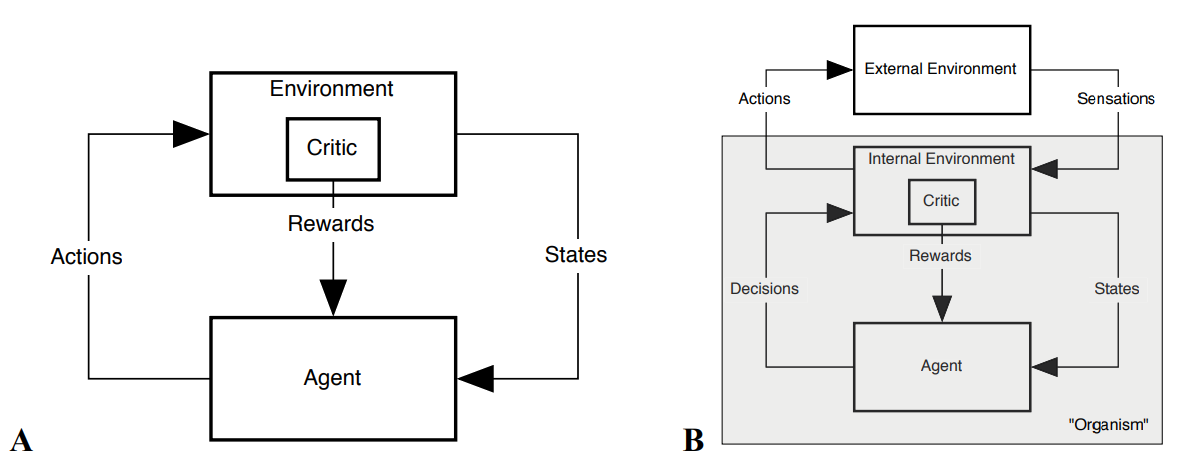
\includegraphics[width=\textwidth]{Q4-Internal-External-Environment.png}
	\caption{Agent-Environment Interaction in RL. \textbf{A}: The usual view. \textbf{B}: An elaboration. \textit{Sourced from \cite{chentanez2005intrinsically}}.
	\label{fig:Internal-External}

\end{figure}

\newpage

\printbibliography


\end{document}
